% last updated in April 2002 by Antje Endemann
% Based on CVPR 07 and LNCS, with modifications by DAF, AZ and elle, 2008 and AA, 2010, and CC, 2011; TT, 2014; AAS, 2016

\documentclass{llncs}
\usepackage{graphicx}
\usepackage{amsmath,amssymb} % define this before the line numbering.
\usepackage{ruler}
\usepackage[dvipsnames]{xcolor}
\usepackage{subcaption}
\captionsetup{compatibility=false}
\usepackage{xcolor}
\usepackage[width=122mm,left=12mm,paperwidth=146mm,height=193mm,top=12mm,paperheight=217mm]{geometry}
\usepackage{multirow}
\usepackage{algorithm}
\usepackage[]{algpseudocode}
\newcommand{\jason}[1]{\textcolor{orange}{\textbf{JASON: #1}}}
\newcommand{\madan}[1]{\textcolor{red}{#1}}

\begin{document}
% \renewcommand\thelinenumber{\color[rgb]{0.2,0.5,0.8}\normalfont\sffamily\scriptsize\arabic{linenumber}\color[rgb]{0,0,0}}
% \renewcommand\makeLineNumber {\hss\thelinenumber\ \hspace{6mm} \rlap{\hskip\textwidth\ \hspace{6.5mm}\thelinenumber}}
% \linenumbers
\pagestyle{headings}
\mainmatter
\def\ECCV18SubNumber{1816}  % Insert your submission number here

\title{TARP: Tensorflow-based Activity Recognition Platform} % Replace with your title

\titlerunning{TARP: Tensorflow-based Activity Recognition Platform}

\authorrunning{Eric Hofesmann, Madan Ravi Ganesh, \and Jason J. Corso}

\author{Eric Hofesmann, Madan Ravi Ganesh, \and Jason J. Corso}
\institute{University of Michigan}
\newcommand{\acro}{TARP}
\newcommand{\model}{\textit{Model submodule}}
\newcommand{\checkpoint}{\textit{Checkpoint submodule}}
\newcommand{\metrics}{\textit{Metrics submodule}}
\newcommand{\data}{\textbf{Data Input Block}}
\newcommand{\exec}{\textbf{Execution Block}}

\maketitle

\begin{abstract}
\keywords{}
\end{abstract}

\section{Introduction}
\label{sec:intro}

\section{Overview of \acro}
\label{sec:overview}

\begin{figure}[b!]
\centering
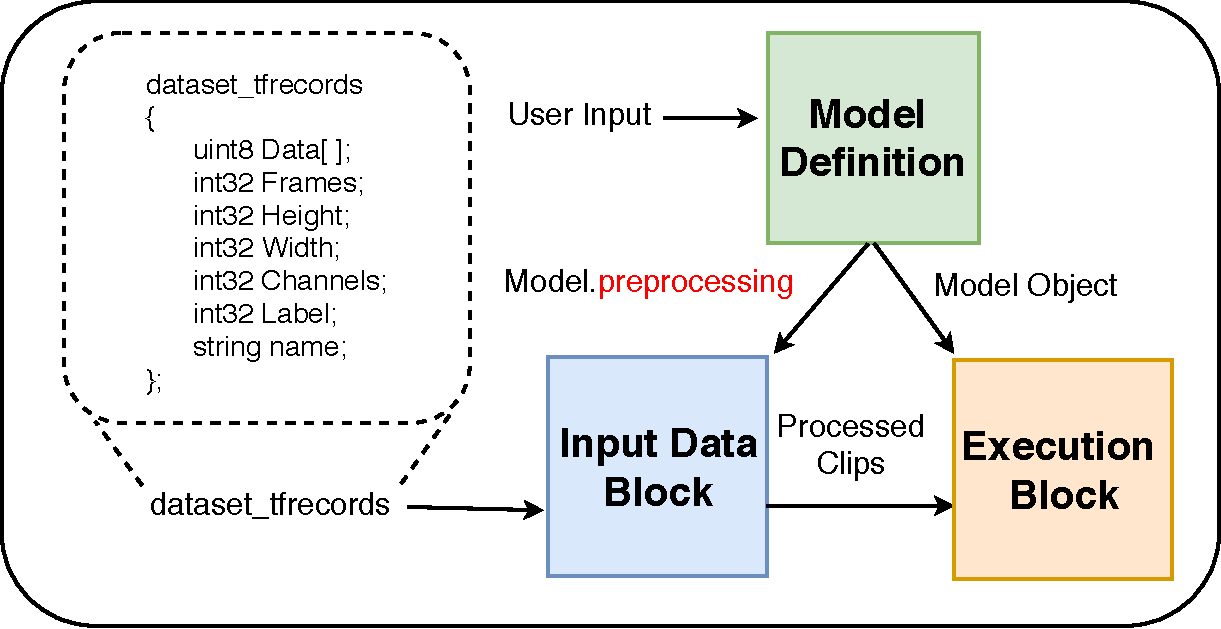
\includegraphics[width=0.8\textwidth]{images/overview.pdf}
\caption{Illustration of the two main components of \acro}
\label{fig:overview}
\end{figure}

\acro~is comprised of two main components, 1) the data input block, and 2) the execution block, as shown in Fig.~\ref{fig:overview}. 
The pipeline contained within the data input block can be divided into three simple stages,
\begin{enumerate}
\item Read video data from disk
\item Extract the desired number of clips from a given video
\item Preprocess the frames of clips using a selected model's preprocessing strategy.
\end{enumerate}
The execution block houses all of the code required to setup, train, test as well as log the outputs of a chosen model.
This includes defining the layers that comprise the model, training the model up to a predetermined number of epochs, saving parameter values of a model are regular intervals and finally testing the performance of the trained model over a variety of recognition metrics.
The following sections provide an in depth discussion of the setup and structure of various components of the platform.

\section{Input Data Block}
\label{sec:ipblock}
Included in the input pipeline are all of the steps required to pass a video into a model in the proper format.
The three stages of the input pipeline, including reading video data, extracting clips, and preprocessing clips, are detailed below.

\begin{figure}
\centering
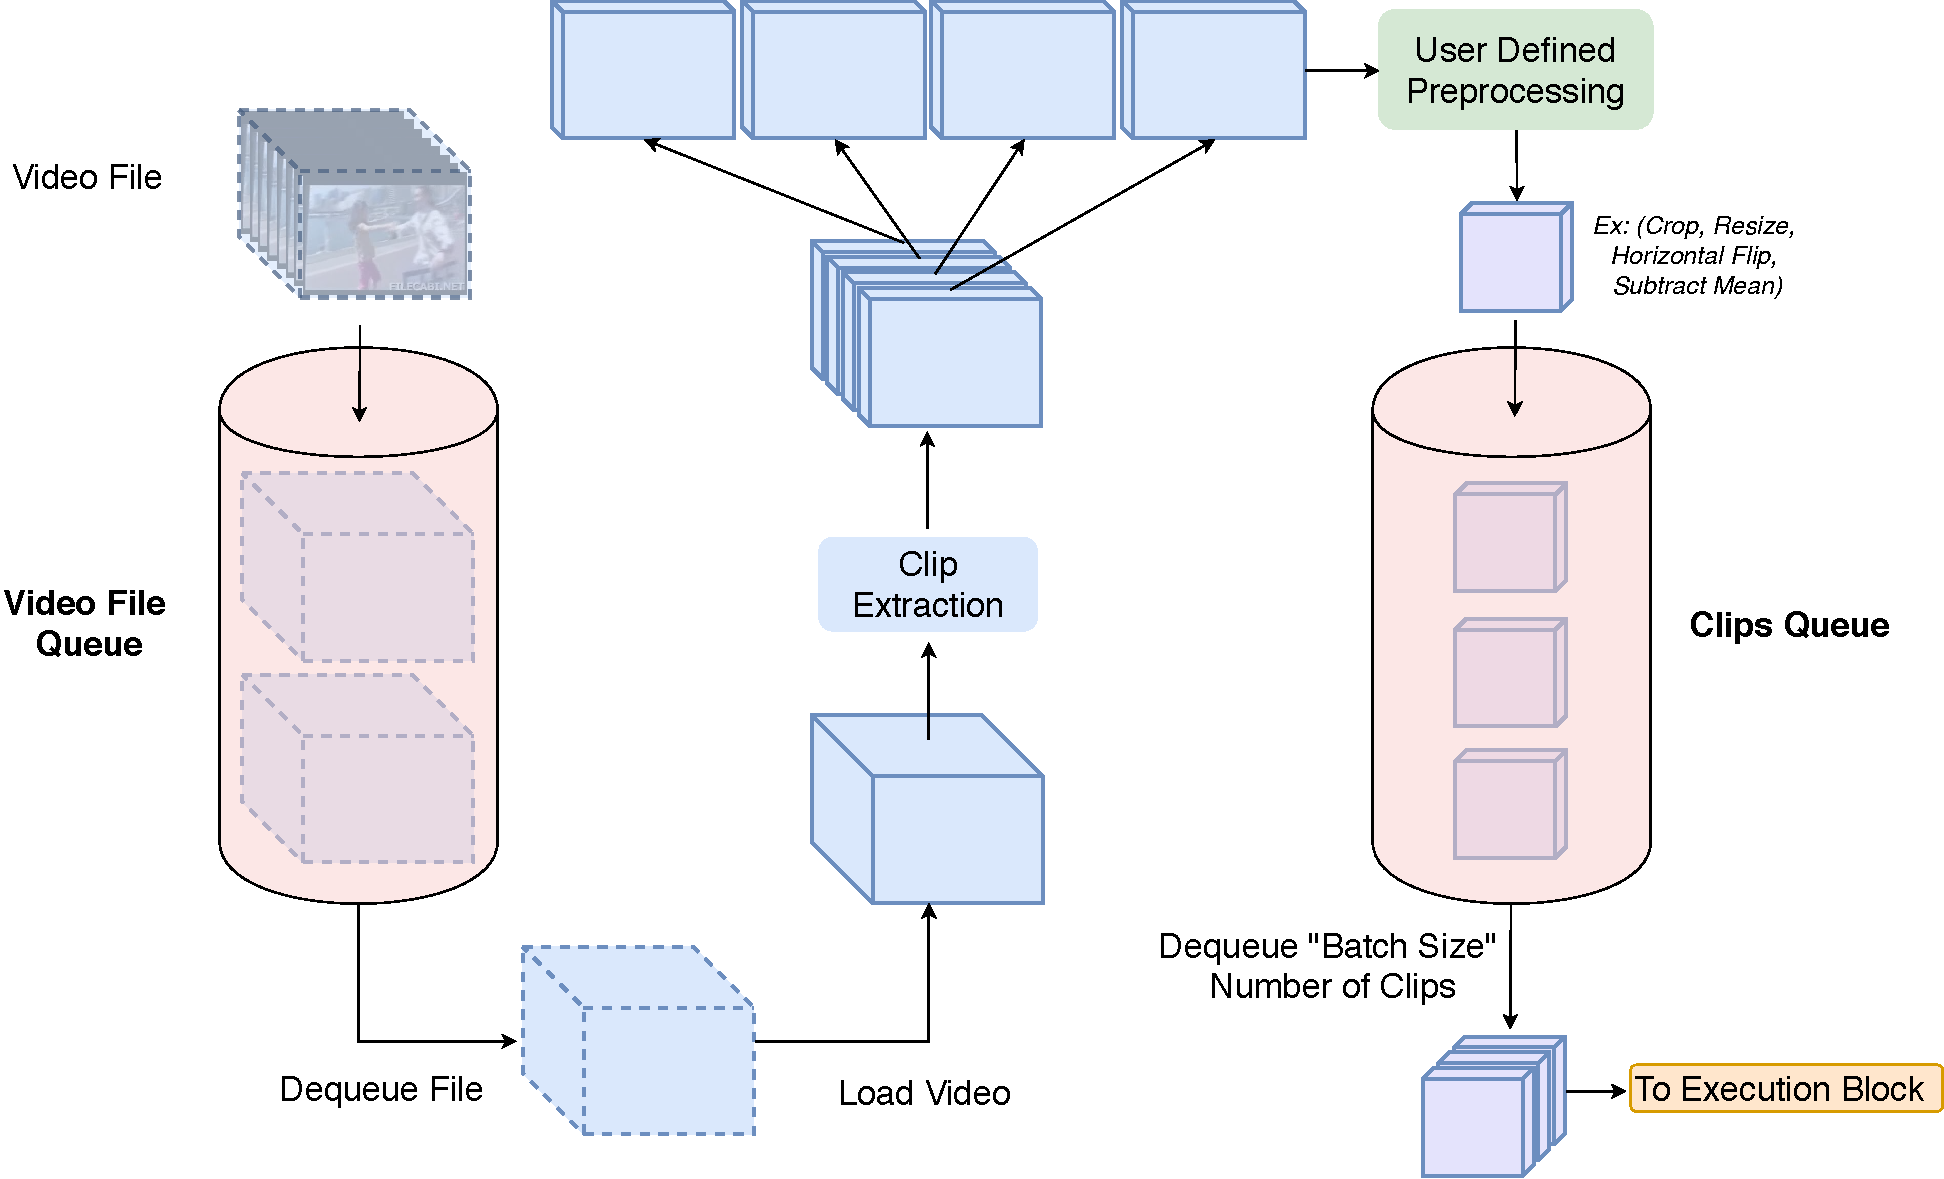
\includegraphics[width=1.0\columnwidth]{images/ip_pipeline.pdf}
\caption{This figure depicts the data flow from loading video files to passing a processed batch of clips into the specified model.
The input pipeline revolves around two separate queues, one queue for storing file names of all tfrecords in the specified dataset and another queue for storing processed clips waiting to be passed to the model.
During runtime, the video file queue gets filled with all tfrecords filenames, which then get dequeued one by one.
The corresponding video to that file gets loaded into the system and it gets broken down into clips as described in Sec.~\ref{sec:extractclips}.
Each clip then gets individually preprocessed according to a set of user defined steps as described in Sec.~\ref{sec:modeldesc}.
The processed queues then get loaded into the \texttt{\textcolor{ForestGreen}{clips\_queue}} so that exactly one \texttt{\textcolor{ForestGreen}{batch\_size}} of clips is available to be loaded into the model.}
\label{fig:ip_block}
\end{figure}


\subsection{Read video data}
\label{sec:readdata}
In \acro, video data is stored in the form of tfrecords files.
These files can be generated using the provided code given that the original video datasets have been acquired.
The contents of these files include the video height, width, channels, number of frames, BGR data, name of the video file, and the label of the action class related to the video.
Video data is stored in BGR format due to the use of OpenCV for converting the given video files to python arrays.
However, the first step of the input pipeline after reading in the tfrecords data is to convert the video to RGB.

Reading tfrecords files is accomplished through the use of a \texttt{\textcolor{ForestGreen}{tfrecord\_file\_queue}} which stores the names of all tfrecords in the requested dataset split.
Enqueue and dequeue operations to this queue are built into the tensorflow graph to allow for efficient parallel data loading.
After individuals are able to be loaded from this queue, these videos must now be broken down into clips and preprocessed.

To allow for the loading of multiple clips for each loaded video, another FIFO queue is added to the pipeline to store individual clips.

Note: When loading the dataset HMDB51, videos are stored in a 30 frames-per-second (fps) format while most models require 25 fps. A function, \textcolor{red}{\_reduce\_fps} is used to remove every sixth frame from HMDB51 videos in order to reduce the fps.

\subsection{Extract clips}
\label{sec:extractclips}
Certain models, for example C3D~\ref{}, require their inputs to be in the form of multiple clips extracted from a single video.
Fig.~\ref{fig:extract_clips} details the various arguments that are available to break down a video into clips.
These methods shown are able to be used in conjunction with one another to give the user the flexibility needed to extract clips with different shapes and sizes.
 
By default, the clip extraction algorithm is set to process and entire video at a time and only extract clips if the required arguments have been specified.
In addition to the options shown in Fig.~\ref{fig:extract_clips}, \acro~also provides options for random selection of clips.



\begin{figure}[b!]
\centering
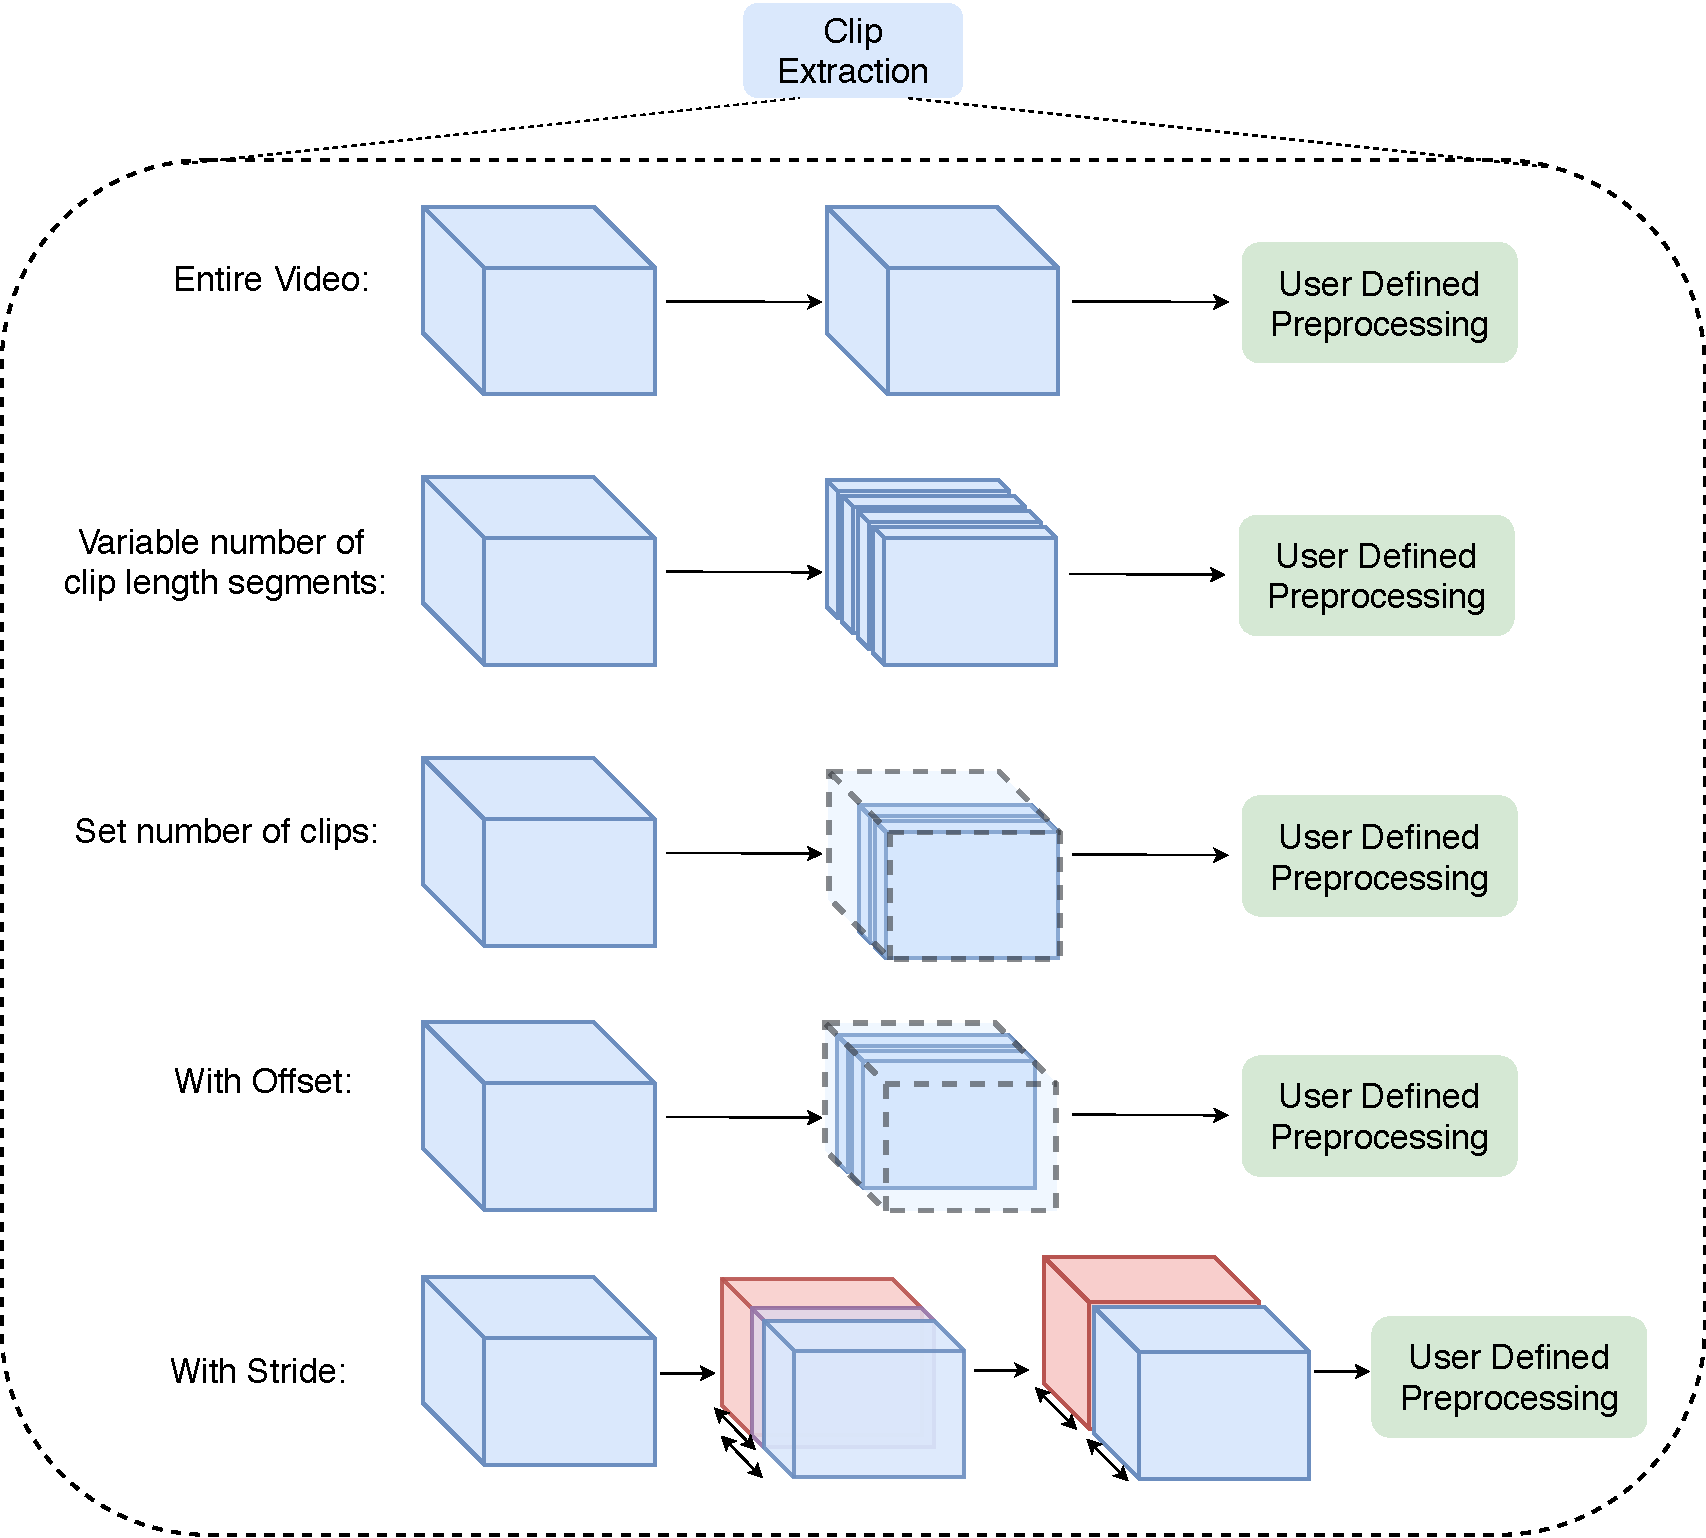
\includegraphics[width=0.8\columnwidth]{images/extract_clips.pdf}
\caption{The clip extraction function allows for videos to be broken into clips according to defined specifications.
Whenever a video has been completely processed and used for training or testing, a new video is loaded from the queue.
The video is then passed through our clip extraction algorithm which enqueues the clips individually into a secondary queue.
Clips are then dequeued from the clips queue according to the number of GPUs being used and the required clip batch size.}
\label{fig:extract_clips}
\end{figure}


\subsection{Preprocess clips}
\label{sec:preprocessclips}
Activity recognition employ a number of various preprocessing methods on a frame or clip-based level.
These can include frame-wise cropping, flipping, and resizing, or clip-wise cropping, flipping, temporal offsets, resampling, and looping.
In order to incorporate these methods as desired per model, we create one or multiple preprocessing files for each model.
The desired preprocessing file for a model can be defined within the model and then called from the inputs call 

\acro~includes implementations of all of these options which can easily be added to a model's preprocessing file.



Note: Due to the nature of tensorflow enqueue operations, errors that occur within an enqueue operation do not properly throw an error. 
The enqueue is simply canceled and an error will occur when the dequeue attempts to access an empty queue. 
This effect occurs within the \texttt{\textcolor{ForestGreen}{clips\_q}} if an error occurs in the user defined preprocessing submodule.
In order to allow proper debugging of the preprocessing submodule, the argument \texttt{\textcolor{ForestGreen}{preprocDebugging}} is available to bypass the \texttt{\textcolor{ForestGreen}{clips\_q}} and see any error tracebacks.
Since the queue used to store clips is removed, the requirement is set that \texttt{\textcolor{ForestGreen}{batch\_size}} must equal \texttt{\textcolor{ForestGreen}{num\_clips}} while debugging.


\section{Execution Block}
\label{sec:execblock}
Training and testing form the two main tenants of the execution block. 
Fig.~\ref{fig:exec_block} illustrates this partition along with the largest submodules present within each part.
Details regarding the flow of data and processes between various submodules and the entire execution block are provided below.

\begin{figure}[t!]
\centering
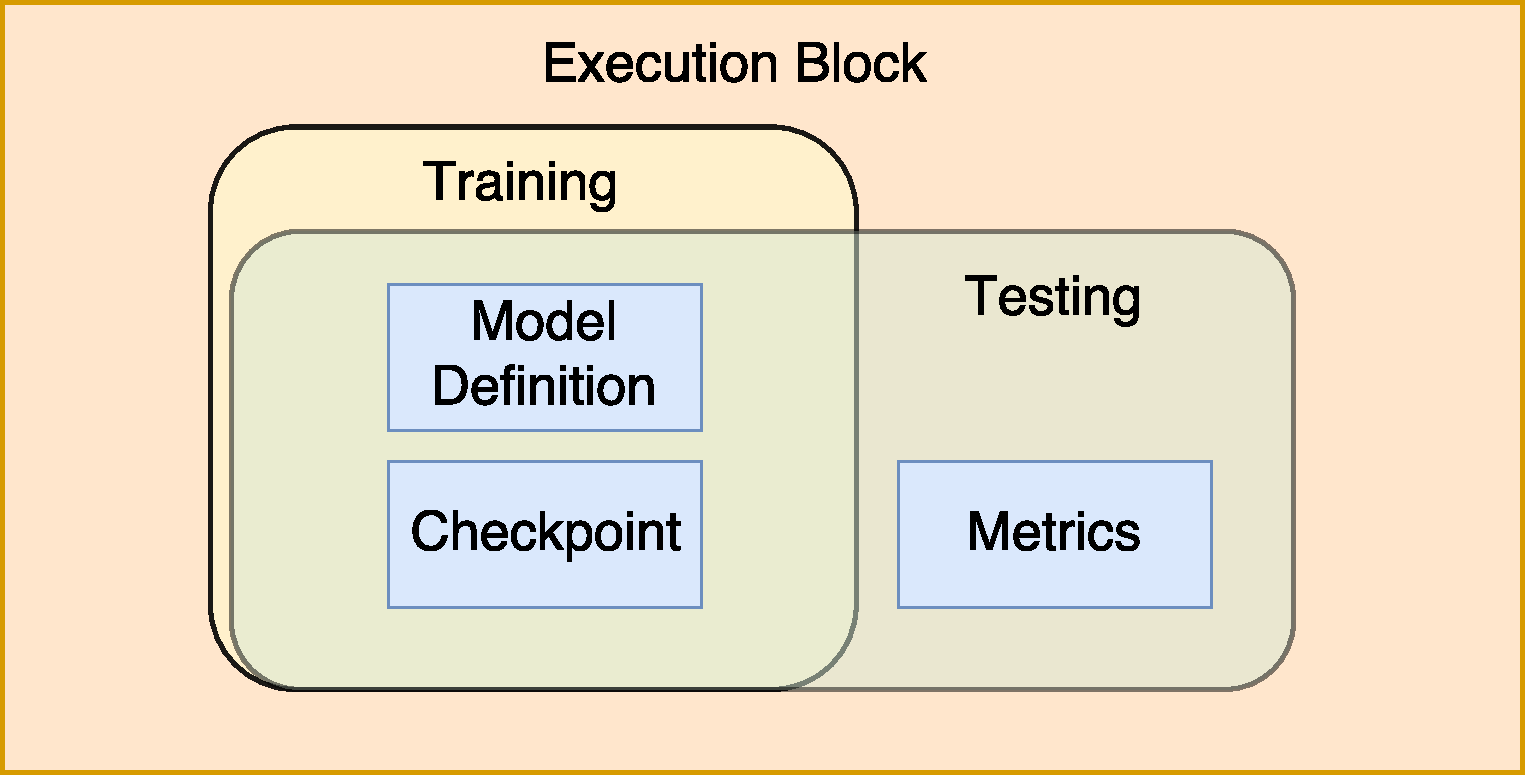
\includegraphics[width=0.8\columnwidth]{images/exec_block.pdf}
\caption{Training and Testing functions are the two major phases within the execution block. Model definitions and checkpoint-based functions are part of both training and testing functions while metrics are calculated after models are tested.}
\label{fig:exec_block}
\end{figure}

\subsection{Training: Algorithmic flow of processes}
\label{sec:training}
Training, within the context of the execution block, follows the process flow outlined in Alg.~\ref{}.
The beginning of every training experiment is aligned with a chosen model. 
Here, basic model parameters such as input/output data dimensions, batch normalization, dropout rate, and etc. are passed into the \model~in order to select and setup a desired model according to well defined prerequisites.

Once the model has been set up, the next step is to ensure that the parameter weights for the chosen model are retrieved. 
If the model has been pre-trained using \acro~and the user desires to further fine-tune the model, then the model parameter's weights from the latest checkpoint will be restored.
By default, the standard pre-trained weights, such as Kinetics~\cite{} for I3D~\cite{}, Sports1M~\cite{} for C3D~\cite{}, ImageNet~\cite{} for ResNet50~\cite{} and TSN~\cite{} are loaded into the model.
Alternatively, a random initialization option, for users to train from scratch is also provided. \\
Note: To ensure that there is a backup when a specified checkpoint is unavailable, the random intialization option is used, with the system providing a warning to the user about the setup used in training.

After the preparation of the model is complete, data tensors are retrieved from the \data.
The main data retuned from \data~are the video frames, their corresponding labels and video names.
With the availability of the model and data, the next stage is creating a copy of the model on the selected number of GPUs within a compute node.
\acro~only supports the extension of a model within a compute node of a cluster. 
Currently, it cannot be distrbute a model across mutiple nodes or split a model across multiple GPUs within a node.

Within each GPU, the inference function of \model~is used to generate a copy of the layer definitions. 
Here, the variable names are re-used to ensure that the same copy of weights are associated throughout all the GPUs.
From each of the model copies, we retrieve a desired layer's output. 
Given that the most common approach to training a network is through the use of logits returned from the final layer, we use the variable logits associated with the last layer to obtain a loss value.
Gradient computation based on the loss calculated is also performed.
Finally, the loss and gradients across all the model copies are accumulated into the loss\_array and gradients\_array respectively.
The contribution of each model copy is weights equally and the final gradient used to update the weights of the model is obtained by taking the average of value stored in the gradients\_array.
The is the final stage in the definition of the tensorflow graph required for training.

\begin{algorithmic}[H]
\Procedure{Training}{}
\State \textbf{Model\_definition}.\textcolor{red}{setup}(model\_params)
\State \textbf{Checkpoint}.\textcolor{red}{load\_param\_weights}(default or specific file)
\State Data, Labels = \textbf{DIB}.\textcolor{red}{load\_data}(expt\_params)
\\
\For{each GPU within given node}
\State \textbf{Model\_definition}.\textcolor{red}{inference}(Data, model\_params)
\State tower\_loss = \textbf{Model\_definition}.\textcolor{red}{loss}(Labels, returned\_logits)
\State tower\_gradients = gradients(tower\_loss)
\State loss\_array.store(tower\_loss)
\State gradients\_array.store(tower\_gradients)
\EndFor
\\
\State grad = average\_gradients(gradients\_array)
\State train\_op = apply\_gradients(grad)
\\
\While{no\_videos\_loaded \textless~(total\_epochs $\times$ videos\_in\_dataset)}
\State \textbf{Checkpoint}.\textcolor{red}{save}() @ regular intervals
\State sess.run(train\_op)
\State update(no\_videos\_loaded)
\EndWhile
\EndProcedure
\end{algorithmic}

After the tensorflow graph for training has been defined, the next step is to execute the graph. 
Usually, models are trained for a typical number of epochs, iterations over the entire dataset.
Within each epoch, based on a set frequency of iterations, we save the model parameter's weights using the save function within \checkpoint.
Additionally, we use a tensorboard logging system to record the loss, training accuracy, and training time along with any specified model parameters at every iteration.
The main operation that gets executed within each iteration is the train\_op.
It is important to note that during the setup of the experiment, \acro~ offers adaptive learning rate control which steps down the learning rate by a factor of $0.1$ when the loss plateaus.



\subsection{Model Description Submodule}
\label{sec:modeldesc}
\begin{figure}[b!]
\centering
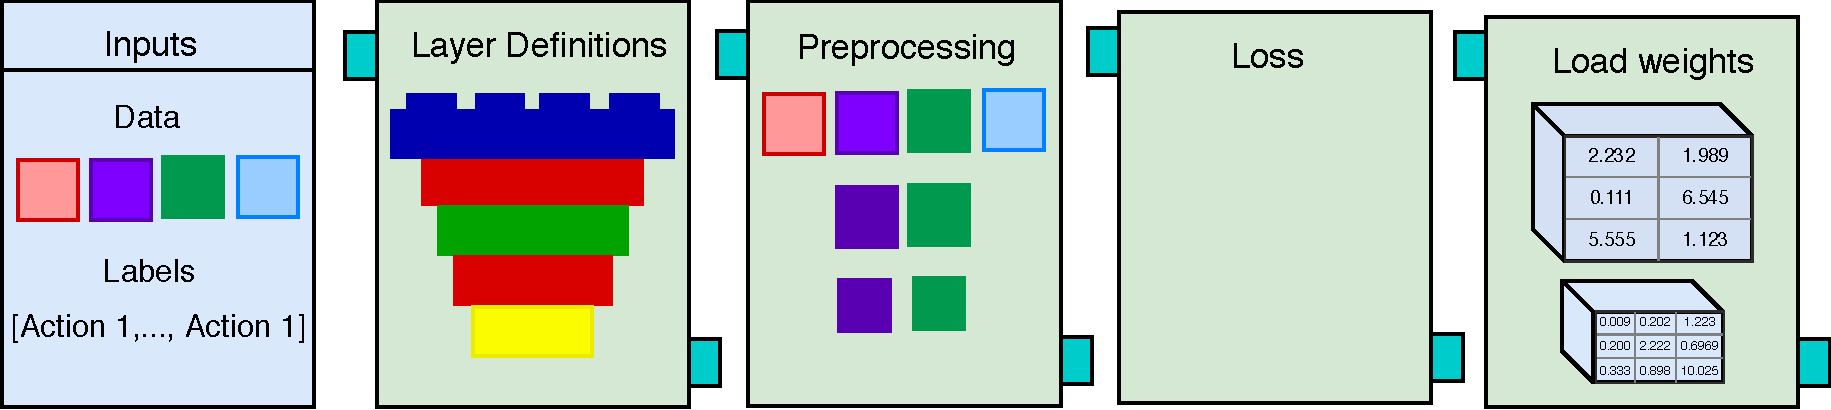
\includegraphics[width=\columnwidth]{images/model_submodule.pdf}
\caption{}
\label{fig:model_submodule}
\end{figure}

The class definition of a model within \acro~can be divided into four main components as shown in Fig.~\ref{}. 
The first step to incorporating a model in \acro~is to define the network architecture within an \textcolor{red}{inference} function.
The layers used must strictly be called from within the set of definitions provided within the \textcolor{blue}{layer\_utils} file.
This ensures that layer definitions are not specific to any network and become available to all models defined within \acro.
Further, it is essential that the inference function returns the outcome of any and all desired layers from within the defined network.
Any accompanying functions to help quickly and/or recursively define a network can be added outisde of the inference function.

Once the network has been defined, the next step is to setup the network's desired preprocessing formulation.
Concrete definitions of each preprocessing step can be included in a separate file.
We provide a standard list of preprocessing functions within the \textcolor{blue}{preprocessing\_utils} file that can be used to construct the entire preprocessing pipeline.
The expected output from a preprocessing function is the preprocessed input data.
Multiple preprocessing pipelines can be included within the same model with the use of the simple \textit{if-else} construct to quickly expand a model's abilities. 
Within the model definition file, it is sufficient to import and call a preprocessing method defined in the adjacent file.

In \acro, we attach the definition of any loss to a model to avoid cluttering and increasing the complexity of the main training file.
Thus, a basic loss function needs to be defined within a models class, with the expected return being logits.
However, the basic loss function can altenratively be used to call different loss functions by using the internally defined \texttt{\textcolor{ForestGreen}{loss\_type}} keyword.

The final and optional component of any model definition within \acro~is the definition of \textcolor{red}{load\_default\_weights} function.
This function is defined to ensure that a predetermined set of weights can be loaded onto the network defined.
The explicit rules required to define the layer names and ensure their respective weights can be assigned are provided in Section~\ref{sec:checkpoint}.
The final values returned by this function are the parameter weights loaded from an external file. 

In order to quickly define and integrate any model into \acro's pipeline, we provide a template file named \textcolor{blue}{models\_abstract.py} which provides the outline for the user to quickly fill out the inference, preprocessing, loss and load weights functions.
A separate file named \textcolor{blue}{models\_preprocessing\_template.py} provides a template for defining the preprocessing pipeline.

Note: 1) Any model defined must be placed within the models folder under a directory with the same name as that of the model,
2) No explicit model class attributes can be added to a specific model. Instead, they must be added to the model\_abstract.py file and made available to any and all model definitions within \acro.
The models that come standard with \acro~include the state-of-the-art activity recognition architectures I3D~\cite{}, C3D~\cite{}, ResNet50~\cite{}, and TSN~\cite{}.

\subsection{Checkpoint Submodule}
\label{sec:checkpoint}

\subsection{Testing: Flowchart of processes}
\label{sec:testing}

Testing begins similarly to training in that a specified model gets defined and initialized according to given parameters.
The model parameters during testing are identical to those used to instantiate a model during training.
Other input arguments that do exist when testing that are not used during training include \texttt{\textcolor{ForestGreen}{metrics\_method}}, \texttt{\textcolor{ForestGreen}{return\_layer}}, and \texttt{\textcolor{ForestGreen}{avg\_clips}}.

After a model object has been instantiated, the model weights are loaded.
The option exists to either load the weights from the default weight file specified within the \textbf{Model Submodule} or to initialize the model to random weights if that is desired.
Most commly, however, the \textbf{Checkpoint Submodule} is used to load the checkpoints of a model that has been trained from scratch or fine-tuned.

Once the model weights are accessible, the dataset will be loaded into the system following the process described in the \textbf{Data Input Block} in Sec.~\ref{sec:ippipeline}.
Videos are not shuffled when being loaded for testing so that all testing instances are directly comparable.
The shape of this input data is set to allow for any number of different videos or multiple clips of a single video to be loaded for testing.
More specifically, the \texttt{\textcolor{ForestGreen}{batch\_size}} of input data can be used to load multiple clips of a single video in order to determine a consensus across these clips which will act as the prediction for the entire video as explained in C3D~\cite{}.
In addition, this \texttt{\textcolor{ForestGreen}{batch\_size}} parameter can also load multiple videos simultaneously if videos are broken into a number of clips which is smaller than the batch.
No models currently use this multiple video functionality for testing, videos are loaded one at a time for testing and only batched for training, but it is available if needed in the future.

Before the data can be loaded into the model, the model must first be copied onto the GPU. 
While only a single GPU is used for testing, a GPU list can still be given to \acro~to determine which GPU the testing instance will be assigned to.
If the list contains more than one GPU device id, the first element in that list will be used.
The process of copying the model to the GPU is based around the \textbf{Model\_definition.}\textcolor{red}{inference} call which will return the output of the layer specified in the \texttt{\textcolor{ForestGreen}{return\_layer}} argument.
By default, the layer that will be returned by \textbf{Model\_definition.}\textcolor{red}{inference} are of the shape [\texttt{\textcolor{ForestGreen}{batch\_size}}, \texttt{\textcolor{ForestGreen}{sequence\_length}}, \texttt{\textcolor{ForestGreen}{output\_dimensions}}] and then converted to action class predictions using the softmax function.
This shape is only required when the \texttt{\textcolor{ForestGreen}{logits}} layer is returned from the \textcolor{red}{inference} call and the application of softmax is dependent on the \texttt{\textcolor{ForestGreen}{useSoftmax}} argument.
With the model output acquired, the final stepis of preparation for testing is to set up the output directory structure, the \textbf{Metrics Submodule} detailed in Sec.~\ref{sec:metrics}, and to load weights into the model as described in the \textbf{Checkpoints Submodule} in Sec.~\ref{sec:checkpoint}.

The testing block iterates through the \texttt{\textcolor{ForestGreen}{num\_vids}} specified which generally includes an entire testing split of a dataset.
Within this block, the tensorflow session is run to extract the model's \texttt{\textcolor{ForestGreen}{output\_predictions}}, ground truth \texttt{\textcolor{ForestGreen}{labels}}, and all video \texttt{\textcolor{ForestGreen}{names}} in this batch.
If the \texttt{\textcolor{ForestGreen}{avg\_clips}} argument has been specified, then the \texttt{\textcolor{ForestGreen}{output\_predictions}} are averaged over their first dimension which is \texttt{\textcolor{ForestGreen}{batch\_size}} or in this case, the number of clips loaded for this testing iteration. 
A tracker counts the number of videos that have been loaded using the video \texttt{\textcolor{ForestGreen}{names}} output.
The \texttt{\textcolor{ForestGreen}{output\_predictions}} and ground truth \texttt{\textcolor{ForestGreen}{labels}} are then fed into the \textbf{Metrics Submodule} for logging and storing.
Finally, the thread coordinator for the input queues is stopped and the all predictions from the \textbf{Metrics Submodule} are saved as a numpy format.


\subsection{Metrics Submodule}
\label{sec:metrics}

\begin{figure}[t!]
\centering
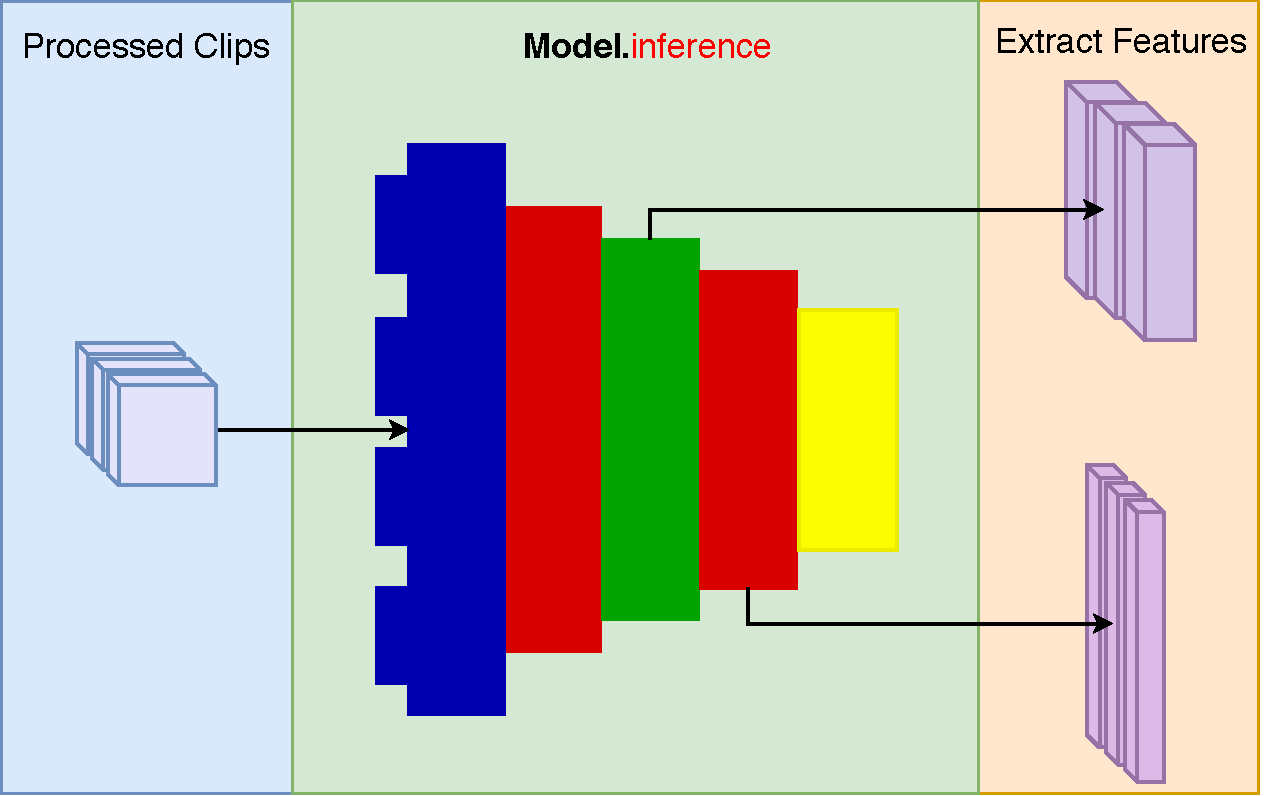
\includegraphics[width=0.7\columnwidth]{images/extract_features_h.pdf}
%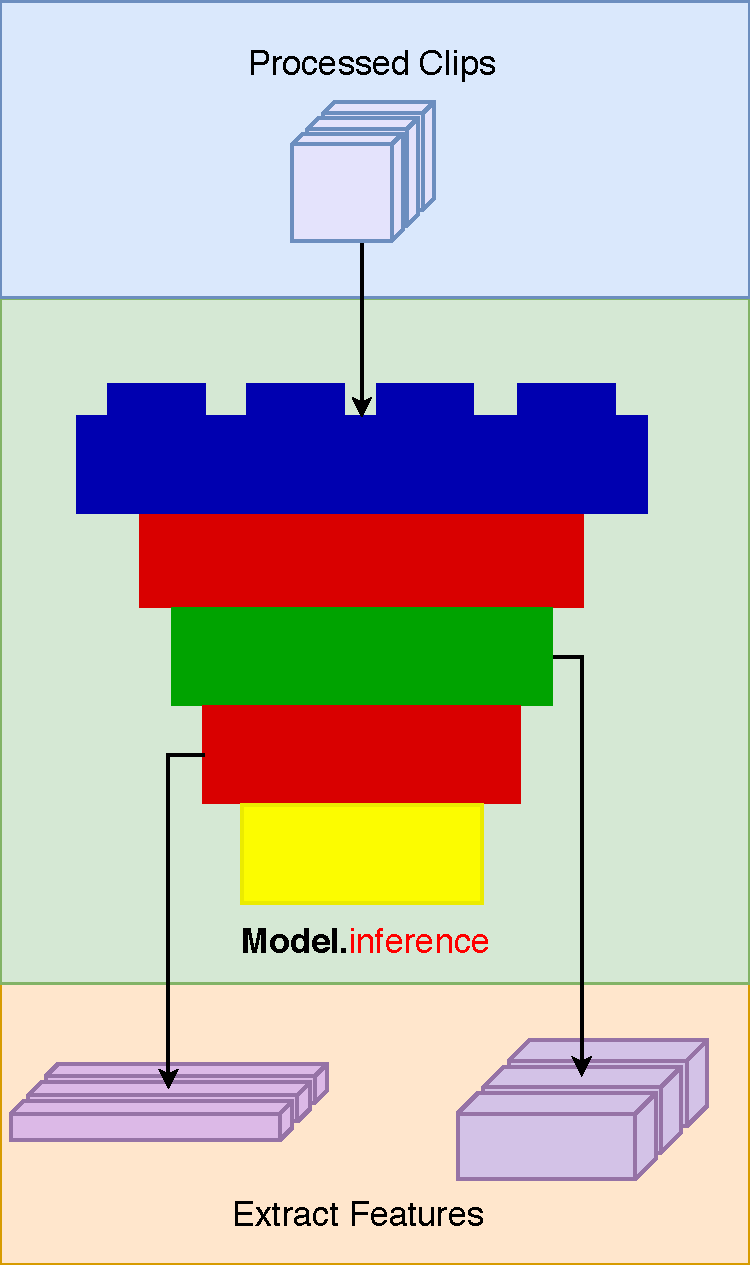
\includegraphics[width=0.3\columnwidth]{images/extract_features_v.pdf}
\caption{}
\label{fig:extract_features}
\end{figure}

\acro~offers a \textbf{Metrics Submodule} for testing and logging the activity recognition performance of a model as well as extracting features from a model. 
This \textbf{Metrics Submodule} is incorporated in the testing pipeline as a class which gets instantiated in \textcolor{blue}{test.py}.
During testing, the output prediction, correct label, and name of each video which is loaded and passed through the model gets stored in this object during every iteration.
These performance metrics and other temporary data gets stored in an hdf5 file format and then deleted at the end of each testing session.
Hdf5 files are used for storing large amounts of temporary data due to their quick reading and writing capabilities.
Just before getting deleted, all relevent testing outputs are saved as numpy files.
Additionally, during testing, the chosen metric and any other specified varaible will be logged automatically using tensorboard.

Available performance metrics include average pooling, last frame prediction, and training a linear SVM classifier.
Average pooling is a common technique which uses the softmax predictions of a model's outputs and averages them across all frames of an input video.
From these predictions, the maximum value is used as the overall class prediction for that video.
The outputs of models can vary in shape so we standardize them to be in the form of [\texttt{\textcolor{ForestGreen}{batch\_size}}, \texttt{\textcolor{ForestGreen}{sequence\_length}}, \texttt{\textcolor{ForestGreen}{number\_of\_classes}}].
The \texttt{\textcolor{ForestGreen}{batch\_size}} parameter slightly changes meaning depending on the model being used.
For example for C3D, multiple clips can be loaded for a single video, the average can then be taken across all of these clips while the temporal dimensionality gets reduced from 16 frames to 1, removing the need for any average pooling or last frame prediction. 
On the other hand, TSN would take multiple videos and refer to each as a single clip, thus the batch of different videos would each be logged separately.
\acro~is robust enough to handle both such cases.
Last frame classification is referenced originally in the ConvNet + LSTM model~\cite{}.
This technique calculates the argmax of solely the last frame of the input clip.
In addition to these metrics which directly classify the output of a model, \acro~also provides the option of training a linear SVM classifier based off of features extracted from any user specified layer within the model.
A linear SVM was used to classify video in the UCF101 dataset in C3D~\cite{}

Features can be extracted for a multitude of reasons other than just to train a linear SVM.
This quality allows \acro~to accomplish more than just activity recognition.
Any of the state-of-the-art models that have been implemented, or even any custom model, can be used for feature extraction.
With any dataset that has been converted to the proper tfrecords format, the correct input arguments allow the user to extract features from any layer in any available model.
Due to the large size that features can become over modern datasets with thousands and even millions of videos, it is crucial to be able to read and write them to memory quickly which is why we use an hdf5 file format for writing this data.




\section{Benchmarks}
\label{sec:benchmarks}

\clearpage

\bibliographystyle{splncs}
\bibliography{egbib}

\end{document}

\grid
\grid
\grid
\grid
\grid


